\section{Network Visualization and Embeddings}
\label{sec:network_visualization}

Drawing complex networks is a fundamentally important problem in network science. Beyond mere aesthetic representation, effective visualization serves as a crucial exploratory tool. It allows researchers to visually identify the macroscopic global structure of the system, visually characterize tightly knit communities, and detect recurring topological patterns or motifs that might be obscured in raw adjacency matrices.

Because human spatial intuition is largely limited to lower dimensions, network representations are typically projected into 2D or, at most, 3D Euclidean spaces. To achieve this, algorithms must translate discrete topological connectivity into continuous spatial coordinates.

\subsection{Force-Directed Layouts}
\label{subsec:force_directed_layouts}

The most common approach to network visualization relies on force-directed graph drawing algorithms. These methods assign physical forces to the nodes and edges, simulating the network as a physical system until it reaches a state of mechanical equilibrium.

\subsubsection{The Spring Embedding Layout}
\label{subsubsec:spring_embedding}

A fundamental approach to defining node coordinates is the spring embedding layout. The core physical intuition is to treat the edges as mechanical springs. The problem is mathematically framed as positioning each node exactly at the center of mass of its immediate topological neighbors.

For a node $i$, its coordinate $X_i$ is calculated as the weighted average of the coordinates of its neighbors $X_j$:
$$X_i = \left( \sum_{j \sim i} A_{ij} \right)^{-1} \sum_{j \sim i} A_{ij} X_j$$

Recognizing that the sum of the adjacency weights corresponds to the degree matrix $D$, we can rewrite this system of equations in matrix form for all nodes $x$:
$$Dx = Ax$$

By rearranging the terms, we introduce the standard network Laplacian operator $L = D - A$:
$$Lx = 0$$

The spatial configuration of the network is therefore intimately linked to the Laplacian spectrum. The trivial solution corresponding to the eigenvalue $\lambda = 0$ places all points at the exact same origin coordinate, which provides no structural information. To obtain a meaningful spatial embedding, we must use the eigenvectors associated with the subsequent non-zero eigenvalues, which provide nontrivial coordinates that optimally preserve the "spring" distances between connected nodes.

\subsubsection{The Kamada-Kawai Algorithm}
\label{subsubsec:kamada_kawai}

While simple spring embeddings center nodes among their neighbors, they often fail to separate disconnected components or distinct clusters effectively. The Kamada-Kawai layout improves upon this by introducing a dual-force system: it balances attractive spring forces acting strictly along the edges with distance-dependent Coulombian repulsive forces acting between all pairs of nodes.

In this model, the attractive spring force depends on the link weight ($a_{ij}$), pulling connected nodes together. Conversely, nodes repel each other with a Coulombian force proportional to assigned node "charges" ($q_i, q_j$), which are frequently defined as proportional to the node's degree.

The net force vector $\vec{F}_{ij}$ between node $i$ and node $j$ is mathematically described as:
$$\vec{F}_{ij} = a_{ij}(\vec{x}_i - \vec{x}_j) - \frac{k \cdot q_i \cdot q_j}{(\vec{x}_i - \vec{x}_j)^2} \vec{u}_{ij}$$
where $k$ is a repulsion constant and $\vec{u}_{ij}$ is the unit vector directing the repulsion.

Because evaluating these forces analytically is complex, the equilibrium state (where the net force on every node is minimized) is achieved through iterative computational simulation.

Standard software packages utilized for computing these complex visual embeddings include MATLAB (via graph object plots), Gephi (optimized for visualizing massive graphs), Cytoscape (extensively used for biological networks due to highly customizable layouts), and the Python NetworkX library.

\subsection{3D Layouts and Dimensionality Reduction: Shrec3d}
\label{subsec:3d_layouts_shrec3d}

Visualizing networks in three dimensions often utilizes techniques grounded in Multi-dimensional Scaling (MDS). If the complete Euclidean distance matrix between all vectors (nodes) is known, MDS uses the principal eigenvectors to completely and accurately reconstruct the original vectors in 3D space. This is exceptionally useful in determining the 3D physical configuration of biological macromolecules like proteins and DNA.

However, a prevalent issue in empirical data is dealing with an \textit{incomplete} distance matrix. For instance, in protein contact maps or Hi-C chromosomal data, we only possess proximity data for the absolute closest spatial nodes.

The \textbf{Shrec3d} algorithm addresses this constraint. It computationally reconstructs the missing elements of the spatial distance matrix by substituting the \textit{shortest path distance matrix} derived purely from the topological network. Empirical testing has shown that this topological approximation works well for reconstructing the 3D shapes of certain proteins.

Despite these successes, defining the exact boundaries of when Shrec3d successfully approximates physical reality remains an open problem. Notable errors emerge in specific protein reconstructions and especially in large-scale DNA structural modeling, where long-range topological paths fail to accurately mimic direct Euclidean spatial folds.

\subsection{Clustering Interpretations: Homophily and Structural Equivalence}
\label{subsec:homophily_structural_equivalence}

When we apply clustering algorithms directly to coordinates generated by algorithms like Kamada-Kawai, we must interpret the results cautiously: we are essentially clustering nodes based on \textit{how we chose to visualize them}. If spring-based coordinates are used, spatial neighborhood and subsequent clustering will heavily depend on the strength of direct node linking.

More broadly, node embeddings and clustering strategies conceptually bifurcate based on two distinct definitions of node similarity:

\begin{itemize}
    \item \textbf{Homophily:} This principle drives clustering based on topological closeness \textit{within} the network. Nodes are considered similar if they are highly interconnected, share short path lengths, and reside within the same densely linked community. It operates on the "birds of a feather flock together" paradigm.
    \item \textbf{Structural Equivalence:} In stark contrast, structurally equivalent nodes may never directly interact or be topologically close. Instead, they are clustered together because they share similar topological features or functional roles within the graph. This includes nodes possessing identical centrality measures or exhibiting identical neighborhood connectivity profiles (e.g., evaluated via the Topological Overlap Matrix, TOM).
\end{itemize}

Choosing between visual/homophilic clustering and structural equivalence depends entirely on whether the researcher aims to identify cohesive interactive groups or functional system roles.

\subsection{Node Embedding: Metric Mapping}
\label{subsec:node_embedding}

While force-directed layouts provide visual intuition in two or three dimensions, a more rigorous and mathematically powerful approach to characterizing networks is through node embedding. The primary aim of node embedding is to systematically remap nodes from the discrete graph domain into a continuous $N$-dimensional vector (metric) space.

By projecting nodes into a high-dimensional vector space, complex topological similarities between nodes are seamlessly translated into measurable geometric distances. This geometric representation is immensely valuable because it allows researchers to apply standard machine learning techniques for clustering, node ranking, and classification. Furthermore, it enables algebraic vector operations (such as summation and subtraction) directly on the node representations, capturing complex relational logic that is impossible to express in a raw adjacency matrix.

\subsubsection{The General Embedding Procedure}
\label{subsubsec:embedding_procedure}

The process of embedding nodes (or equivalently, textual elements like words) follows a structured framework designed to preserve node similarity based on a specific objective function. The general architecture consists of three fundamental components:

\begin{enumerate}
    \item \textbf{Information Extractor:} A mechanism that systematically extracts the key topological or relational information that needs to be preserved from the original graph or text domain.
    \item \textbf{Reconstructor:} A model designed to retrieve or predict the original extracted graph/text information using only the vectors from the new embedding domain.
    \item \textbf{Objective Function:} A mathematical loss function used to train and learn all the parameters involved in the mapping and reconstructor steps.
\end{enumerate}

The simplest working hypothesis for this architecture is a linear mapping. In this scenario, the transformation is governed by an $N \times D$ weight matrix, where $N$ represents the total number of original nodes (or words) and $D$ represents the target dimensionality of the continuous vector embeddings.

\begin{figure}[H]
    \begin{minipage}{0.6\textwidth}
        \centering
        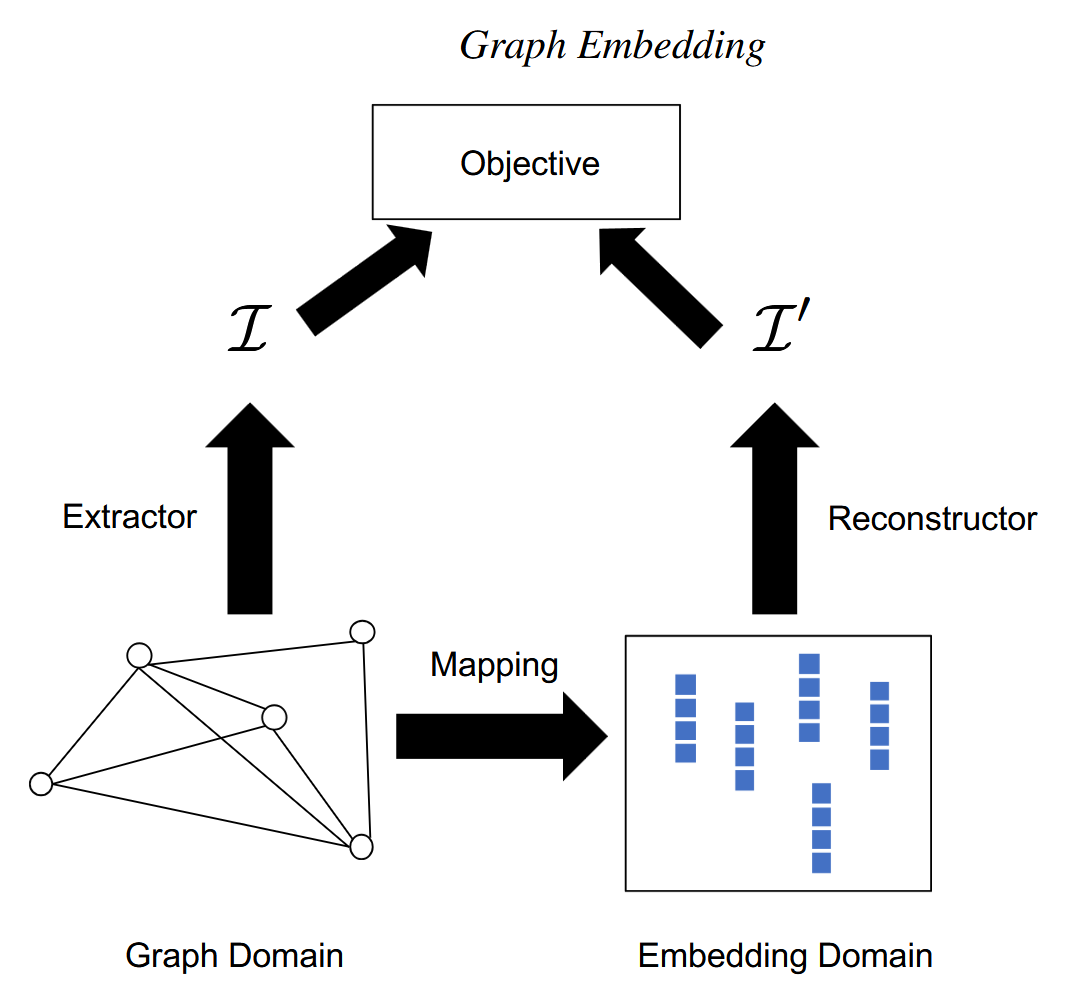
\includegraphics[width=0.8\textwidth]{img/8-node_embedding_framework.png}
    \end{minipage}
    \hfill
    \begin{minipage}{0.35\textwidth}
        \caption{Schematic diagram of the Node Embedding framework. The diagram illustrates the flow from the Graph Domain through the Information Extractor to yield $\mathcal{I}$, which connects to the Objective function. Simultaneously, a Mapping leads to the Embedding Domain, which flows into a Reconstructor yielding $\mathcal{I}'$, which also connects to the Objective function to close the learning loop.}
    \end{minipage}
\end{figure}

\subsection{Word Embedding as a Blueprint: Word2Vec}
\label{subsec:word_embedding_word2vec}

To understand how to embed network nodes, it is highly instructive to look at Natural Language Processing (NLP), which faces a virtually identical problem: embedding words and sentences into dense vectors.

In NLP, words pose significant challenges because they have varying lengths, and morphological similarity (e.g., letter overlap or shared prefixes) does not generally equate to semantic similarity. Because words cannot be easily compared by their explicit structures, researchers developed strategies to embed them based on their contextual usage. This exact strategy—mapping discrete entities based on their contextual surroundings—is directly transferable to embedding nodes in a network.

\subsubsection{Information Extraction: Word Proximity and One-Hot Encoding}

The starting point for text embedding requires a foundational vocabulary. Given a dictionary of $N$ discrete words, the initial representation is a \textbf{1-hot encoding}. Each word is represented as an $N$-dimensional vector containing all zeros except for a single $1$ at the index corresponding to that specific word.

While computationally simple, 1-hot encoding yields trivial and useless metrics: every word vector is perfectly orthogonal to every other word vector, and the Euclidean distance between any pair of words is identical. It contains zero semantic information.

To extract actual relational information, we must analyze "word proximity" by creating a co-occurrence matrix. The text is processed using a sliding window of a fixed size (e.g., 3 words before and 3 words after a target word). For each sentence, a specific word is designated as the \textbf{CENTER}, and the algorithm counts the appearance of other words within the defined \textbf{CONTEXT} window. These counts are aggregated to quantify the relationships $(N_{CEN}, N_{CON})$.

The size of the context window dictates the nature of the learned relationships: a larger window captures broader, more complex topical relationships, but drastically increases the required training time and the volume of data needed.

\subsubsection{Neural Network Reconstruction: CBOW and Skip-Gram}

To transition from raw co-occurrence counts to dense embeddings, a two-layer neural network is trained using one of two primary architectures:
\begin{itemize}
    \item \textbf{Skip-Gram:} The network takes the \textit{center word} as the input and attempts to predict the surrounding \textit{context words} as the output.
    \item \textbf{CBOW (Continuous Bag of Words):} The network takes the surrounding \textit{context words} as the input and attempts to predict the central \textit{target word} as the output.
\end{itemize}

The neural network utilizes two distinct weight matrices. The first is $W$, an $N \times D$ matrix that projects the $N$-dimensional 1-hot encoded inputs into a lower $D$-dimensional hidden layer. The second is $W'$, a $D \times N$ matrix that maps the hidden layer back to the $N$-dimensional output space to generate predictions. It is crucial to note that $W'$ is simply the weight matrix of the second layer and is \textit{not} the mathematical inverse of $W$.

To generate valid probability distributions for the predictions, a Softmax function is applied over the raw output vector $y$:
$$p_i = \frac{e^{y_i}}{\sum_{j} e^{y_j}}$$

\begin{figure}[H]
    \centering
    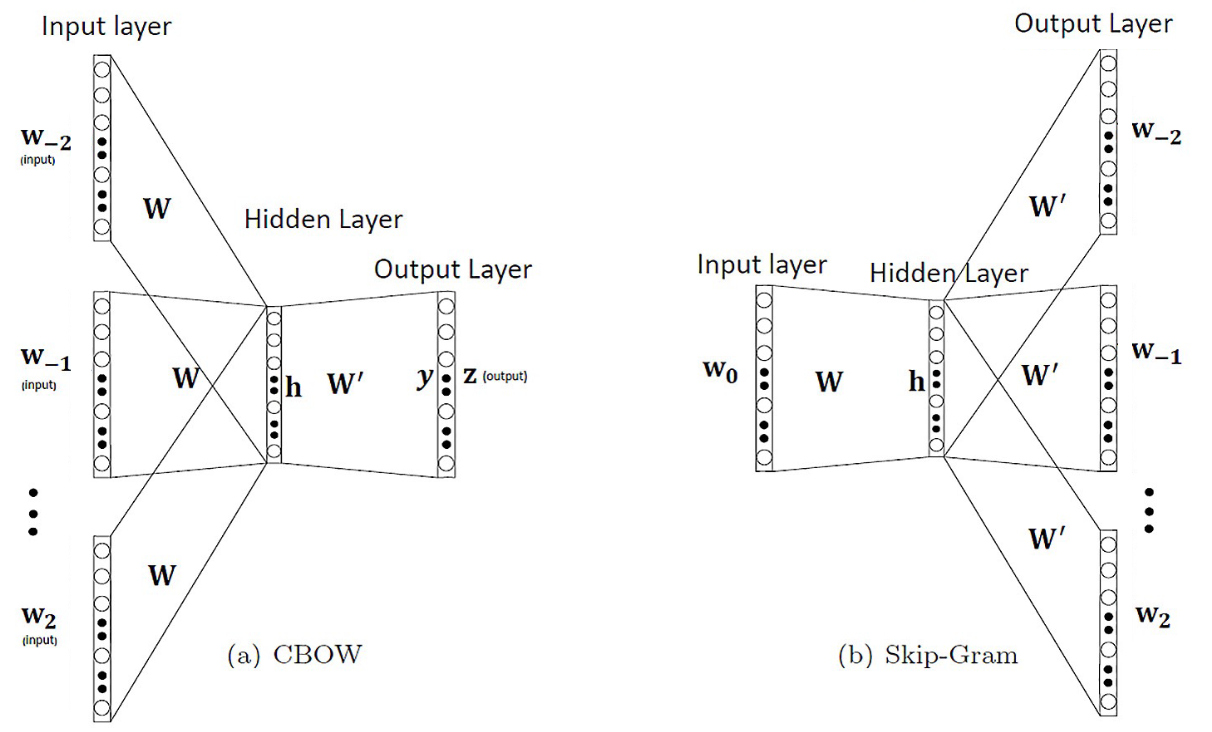
\includegraphics[width=0.7\textwidth]{img/8-cbow_skipgram.png}
    \caption{Schematic diagram illustrating the architectures of CBOW and Skip-Gram. The diagram shows the Input layer (1-hot encoded), the $W$ matrix leading to a $D$-dimensional Hidden Layer ($h$), and the $W'$ matrix leading to the Output Layer with Softmax applied. The CBOW side shows multiple context inputs converging on one output, while the Skip-Gram side shows one input diverging to multiple context outputs.}
\end{figure}

\subsubsection{Objective Function and The Embedding Layer}

The training process relies on semi-supervised learning. There are no external, human-annotated "ground truth" labels; instead, the network learns the "proximity" extracted directly from the sequential structure of the sentences themselves.

The objective function used to evaluate the Softmax output scores (probabilities) against the true outputs is the \textbf{Cross-Entropy (CE)} loss. If $q_i$ represents the true output distribution (derived from actual co-occurrences) and $p_i$ represents the predicted Softmax probabilities, the network seeks to minimize the difference:
$$CE = - \sum_{i} p_i \log q_i$$

\textbf{The critical breakthrough of this architecture is the hidden layer.} The explicit output of the neural network (the context predictions) is ultimately discarded. Instead, the $D$-dimensional hidden layer—specifically the optimized weight matrix $W$—is extracted. The rows of this matrix constitute the final dense \textbf{word embeddings}.

In this framework, we strictly encode \textit{word proximity} within sentences. We do not explicitly encode dictionary definitions. However, because words with similar meanings tend to appear in similar syntactic and contextual positions within sentences, the encoding of \textit{word meaning} emerges as a powerful indirect result. This identical principle is used in network science (e.g., DeepWalk, Node2Vec) where random walks on a graph substitute for sentences, allowing nodes to be embedded based on their topological context.

\subsection{Random Walk-Based Embeddings: DeepWalk}
\label{subsec:deepwalk}

To apply the neural embedding architectures developed for Natural Language Processing (such as Skip-Gram or CBOW) to the domain of complex networks, we require a method to generate linear sequences of nodes that capture the underlying topology. The foundational algorithm that bridges this gap is \textbf{DeepWalk}.

DeepWalk generates these sequences by simulating stochastic processes on the graph, specifically by performing $\gamma$ independent random walks starting from every single node in the network. By doing so, we create a direct structural analogy to text analysis:
\begin{itemize}
    \item \textbf{Sentence:} A generated random walk across the graph.
    \item \textbf{Center Word:} Each specific node visited along the trajectory of the walk.
    \item \textbf{Context:} The surrounding nodes visited within a fixed distance (window size) from the center node during that specific walk.
\end{itemize}

Once this corpus of artificial "sentences" is generated, DeepWalk feeds them directly into a CBOW or Skip-Gram model to reconstruct the center-context relationships, effectively learning continuous vector representations that preserve the neighborhood structure of the graph.

The behavior and computational complexity of DeepWalk are governed by three primary hyperparameters:
\begin{enumerate}
    \item \textbf{Number of random walks per node ($\gamma$):} Dictates the breadth of network exploration. Higher values ensure that the stochastic nature of the walks adequately samples the varied paths available from any given starting point.
    \item \textbf{Walk length ($T$):} Defines the exploration depth. Longer walks capture structural correlations over greater topological distances.
    \item \textbf{Context size ($W$):} The window size within the generated sequence, which defines the strict node proximity depth used by the neural network during training.
\end{enumerate}

\subsection{Second-Order Random Walks: Node2vec}
\label{subsec:node2vec}

While DeepWalk effectively captures network structure, it relies on strict first-order random walks. In a first-order walk, the transition probability of moving from the current node $x(t)$ to the next node $x(t+1)$ is strictly proportional to the link weight between them (rescaled by the current node's degree), without any memory of how the walk arrived at $x(t)$.

\textbf{Node2vec} introduces a more sophisticated, highly flexible approach by employing \textit{second-order} random walks. A second-order walk inherently depends not just on the current node at time $t$, but also on the previously visited node at time $t-1$. This memory allows Node2vec to smoothly interpolate between two extreme topological sampling strategies:

\begin{itemize}
    \item \textbf{Breadth-First Search (BFS):} This strategy restricts the walk to the immediate local neighborhood of the starting node before moving further away. BFS is exceptionally good at capturing \textit{structural equivalence}, grouping nodes that share the same functional role or local structural patterns within the network, even if they are far apart macroscopically.
    \item \textbf{Depth-First Search (DFS):} This strategy encourages the walk to move rapidly away from the initial node, exploring distant regions via long paths. DFS excels at capturing \textit{homophily} and macro-connectedness, grouping nodes that belong to the same large-scale community.
\end{itemize}

\begin{figure}[H]
    \centering
    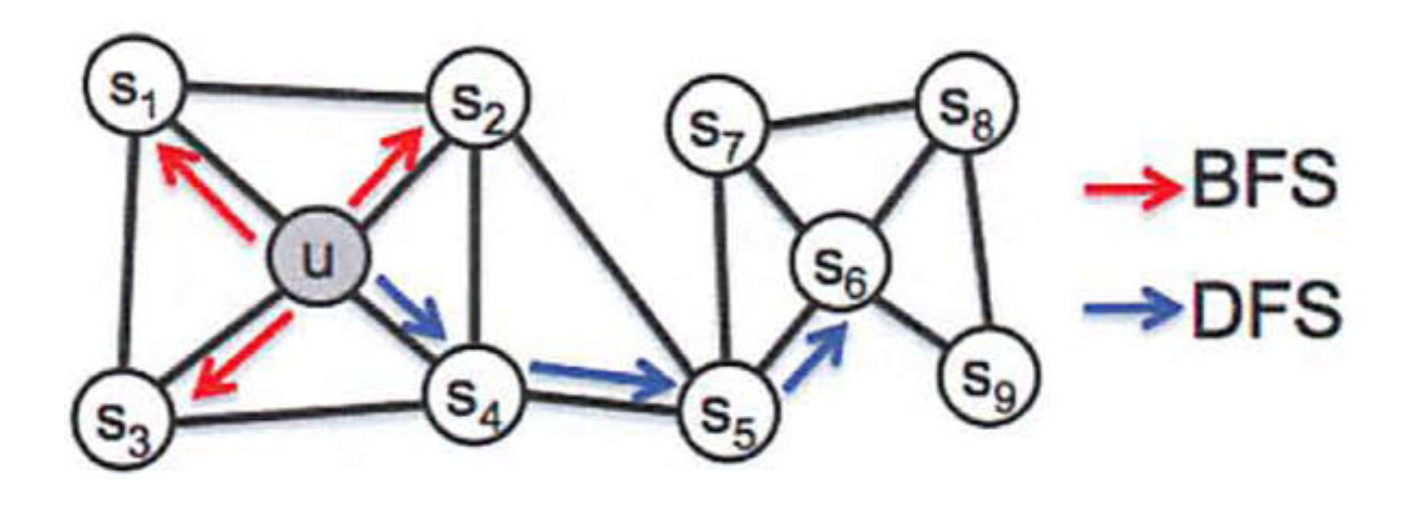
\includegraphics[width=0.8\textwidth]{img/8-bfs_dfs.png}
    \caption{Schematic diagram illustrating the difference between BFS and DFS trajectories in a graph. The central node 'u' is shown with red arrows indicating a BFS trajectory that explores immediate neighbors, while blue arrows indicate a DFS trajectory that extends outward to more distant nodes.}
\end{figure}

\subsubsection{Transition Probabilities and Tuning Parameters}

To mathematically implement this interpolation, Node2vec defines a biased random walk controlled by two hyper-parameters: the return parameter $p$ and the in-out parameter $q$.

Assume the random walk has just traversed the edge from node $t$ (at time step $t-1$) to node $v$ (at time step $t$). The algorithm must now evaluate the unnormalized transition probability $\alpha$ of stepping to a neighboring node $x$ at time $t+1$. This probability is determined by the shortest path distance, $d(t, x)$, between the previous node $t$ and the candidate next node $x$:

\begin{itemize}
    \item \textbf{Case 1: $d(t, x) = 0$ (Backtrack).} The walk evaluates returning directly to the previous node $t$. The unnormalized probability is assigned as $\alpha = \frac{1}{p}$. A high value of $p$ discourages backtracking, pushing the walk outward.
    \item \textbf{Case 2: $d(t, x) = 1$ (Closer/Same Distance).} The candidate node $x$ is an immediate neighbor of both $v$ and $t$ (forming a triangle). The walk stays local, and the probability is assigned a baseline of $\alpha = 1$.
    \item \textbf{Case 3: $d(t, x) = 2$ (Further).} The candidate node $x$ is a neighbor of $v$ but is not directly connected to the previous node $t$. The walk moves further away, and the probability is assigned as $\alpha = \frac{1}{q}$. A low value of $q$ strongly encourages outward DFS exploration, while a high value of $q$ penalizes distant exploration, favoring local BFS behavior.
\end{itemize}

These raw transition weights must, of course, be strictly \textbf{normalized} at each node to form a valid probability distribution before the stochastic step is executed. By fine-tuning the $p$ and $q$ parameters, researchers can highly customize the embedding space to reflect either the homophilic communities or the structurally equivalent roles of the specific complex system under study.

\begin{figure}[H]
    \begin{minipage}{0.6\textwidth}
        \centering
        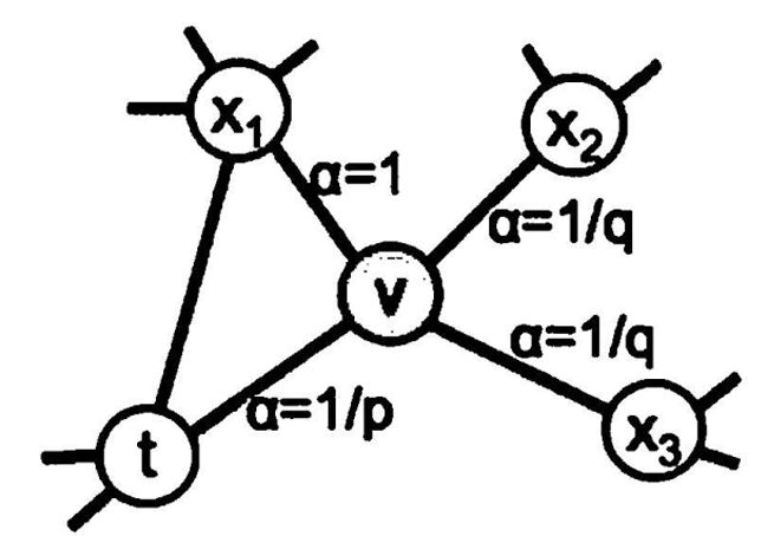
\includegraphics[width=0.8\textwidth]{img/8-node2vec_transition.png}
    \end{minipage}
    \hfill
    \begin{minipage}{0.35\textwidth}
        \caption{Schematic diagram illustrating the transition probabilities in Node2vec. The diagram shows a node 'v' with three outgoing edges: one back to 't' with probability $\alpha = 1/p$, one to 'x$_1$' (a neighbor of both 'v' and 't') with probability $\alpha = 1$, and two edges to 'x$_2$' and 'x$_3$' (further away) with probability $\alpha = 1/q$.}
    \end{minipage}
\end{figure}

\subsection{Applications and Limitations of Node Embeddings}
\label{subsec:embedding_applications_limitations}

The profound advantage of mapping discrete network nodes into continuous $D$-dimensional vector spaces is that it seamlessly bridges graph theory with the massive ecosystem of modern Machine Learning (ML) and Artificial Intelligence (AI) tools.

Once nodes are represented as vectors, several advanced analyses become trivial:
\begin{itemize}
    \item \textbf{Standard ML Tasks:} Nodes can be fed directly into standard algorithms (like K-Means, SVMs, or Random Forests) for robust clustering, node classification, and property regression.
    \item \textbf{Link Inference:} Missing or future links can be predicted with high accuracy by evaluating the geometric similarity (e.g., cosine similarity or Euclidean distance) between two node embeddings.
    \item \textbf{Vector Operations:} We can perform algebraic operations directly on the nodes. For instance, computing the average or the sum of the vector embeddings of a specific group of nodes can yield a highly representative vector defining a topological path or an entire network community.
    \item \textbf{Visualization:} High-dimensional embeddings can be passed through dimensionality reduction algorithms (such as PCA, t-SNE, or UMAP) to project the network structure into clear, informative 2D or 3D visual spaces.
\end{itemize}

\subsubsection{The Transductive Limitation}

Despite their immense utility, it is critical to note a fundamental limitation of methods like DeepWalk and Node2vec: they are inherently \textbf{transductive}.

This means that the embedding mapping works exclusively \textit{within the specific network} it was trained on, and the model holds no internal generalization parameters. The neural network learns a distinct, hard-coded vector for every single unique node present during the training phase. Consequently, if the network evolves—even by the addition of a single new node or edge—the current embedding space cannot intrinsically evaluate it. To embed the new node and maintain relative topological accuracy, the entire random walk generation and neural network training process must be strictly repeated from scratch.

\section{Graph Neural Networks (GNNs)}
\label{sec:graph_neural_networks}

Traditional machine learning algorithms and neural network architectures are primarily designed to operate on regular, Euclidean data structures, such as 1D sequences (text, time series) or 2D grids (images). However, many complex systems are best described by graphs, which reside in non-Euclidean domains. Graph Neural Networks (GNNs) represent a powerful class of deep learning methods specifically designed to bridge this gap. GNNs explicitly exploit the underlying network topology to perform complex learning tasks.

The core functional mechanisms of GNNs revolve around two primary operations:
\begin{itemize}
    \item \textbf{Message Passing and Aggregation:} Systematically transferring and aggregating information (features) contained within the nodes across different local and global topological levels.
    \item \textbf{Graph Structure Learning:} Leveraging these aggregated representations to learn the intrinsic graph structure, which is vital for downstream tasks such as link inference, node classification, and community detection.
\end{itemize}

\subsection{The Convolutional Analogy: CNNs}
\label{subsec:convolutional_analogy}

To conceptually understand how GNNs process network data, it is highly instructive to draw an analogy with Convolutional Neural Networks (CNNs), which are the standard architecture for processing 1D and 2D signals.

\subsubsection{Mechanisms of Convolution}

CNNs integrate multidimensional signals recursively at multiple scales. The fundamental operation is \textbf{masking} (or convolution). This involves the integration of a restricted part of the input data—known as the "receptive field"—with a learnable \textit{kernel} (also referred to as a mask or filter).

Mathematically, this integration is achieved through a scalar or Hadamard (element-wise) product between the input values ($x_i$ or $s_{ij}$) and the learnable weights ($w_i$ or $w_{ij}$) contained within the kernel:
$$ \sum w_i x_i \quad \text{or} \quad \sum w_{ij} s_{ij} $$

Once this linear combination is computed, a nonlinear activation function $\sigma$ (such as ReLU, Sigmoid, or Tanh) alongside a bias term $\beta$ is applied to generate the hidden state output $h$:
$$ h = \sigma\left(\sum w_i x_i + \beta\right) $$

Crucially, multiple different maskings (kernels) can be applied to the exact same input patch simultaneously to extract a diverse set of features.

\subsubsection{Convolution Parameters}

The behavior of the convolutional kernel across the data lattice is governed by three primary geometric parameters:
\begin{itemize}
    \item \textbf{Kernel Size:} The absolute number of elements (e.g., time points in an audio signal, pixels in an image) that are integrated via the weighted product in a single convolution step.
    \item \textbf{Kernel Stride:} The discrete step size or "shift" between one masking application and the subsequent one as the kernel slides across the input data.
    \item \textbf{Kernel Dilation:} A technique used to increase the receptive field of the kernel without increasing the actual number of integrated elements (parameters). It is achieved by interspersing zeros between the active weights in the mask.
\end{itemize}

\begin{figure}[H]
    \centering
    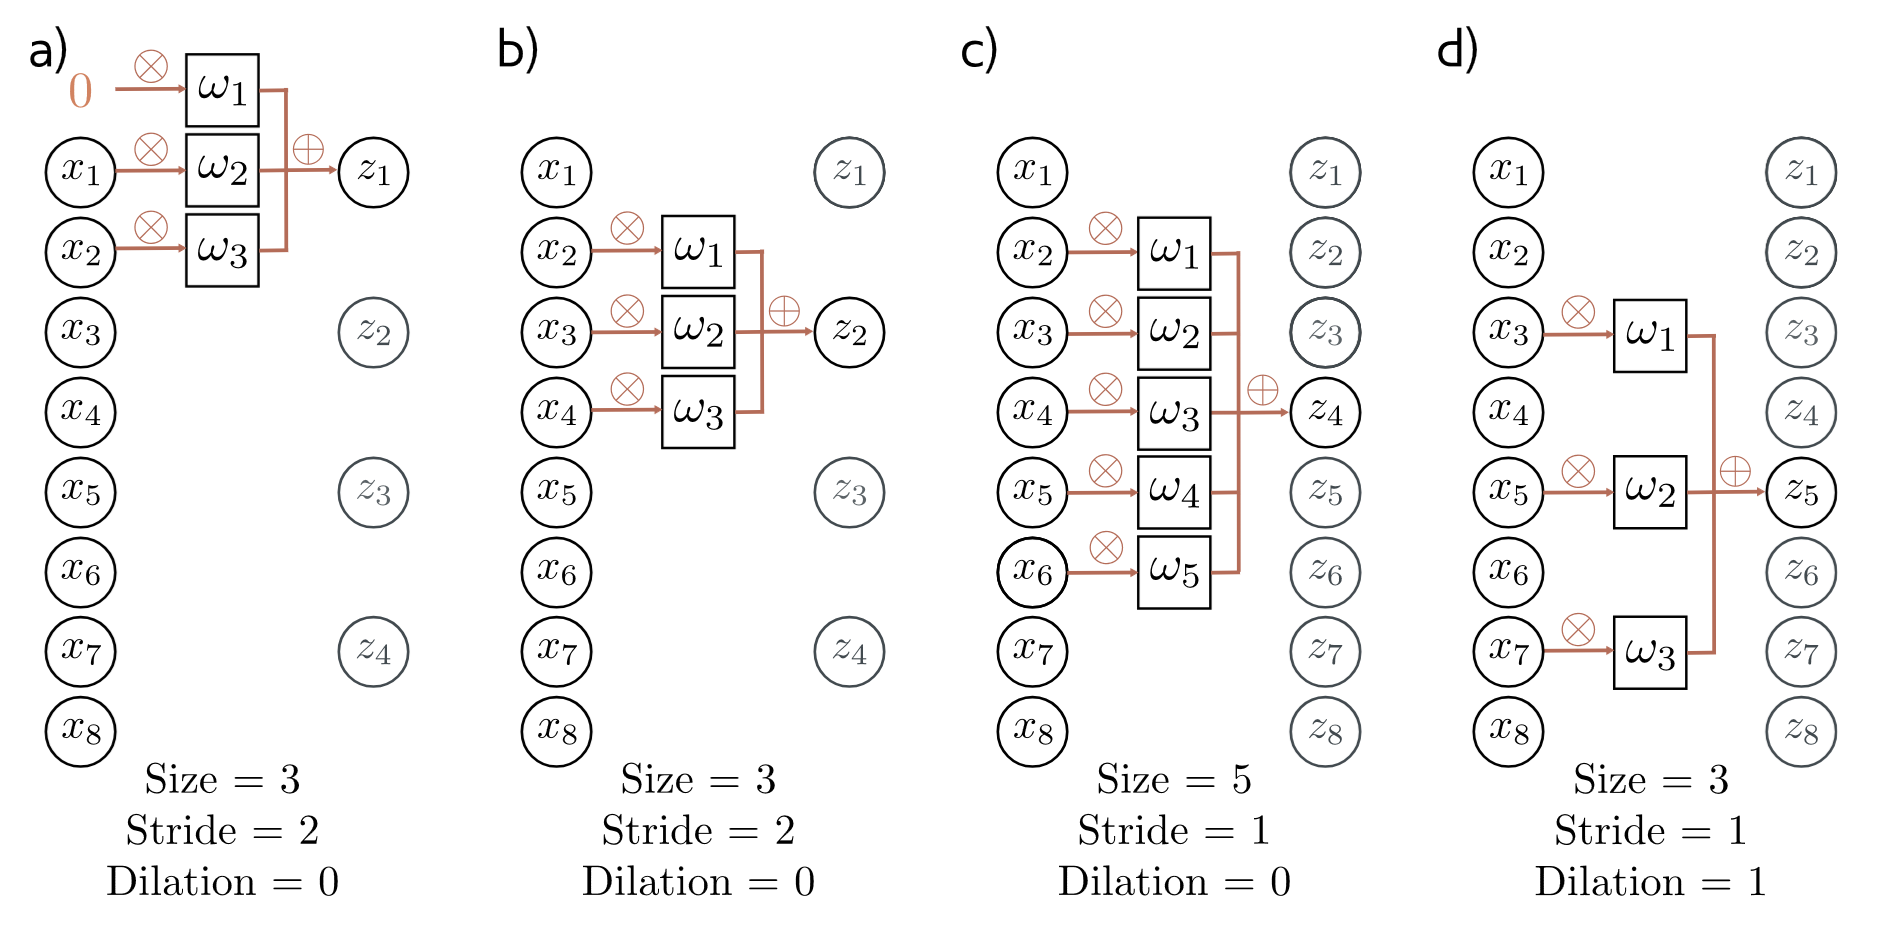
\includegraphics[width=0.8\textwidth]{img/8-convolution_parameters.png}
    \caption{Stride, kernel size, and dilation. (a) With a stride of two we evaluate the kernel at every other position and so the first output z$_1$ is computed from a weighted sum centered at x$_1$ and (b) the second output z$_2$ is computed from a weighted sum centered at x$_3$ and so on. (c) The kernel size can also be changed. With a kernel size of five we take a weighted sum of the nearest five inputs. (d) In dilated or atrous convolution, we intersperse zeros in the weight vector to allow us to integrate over a larger area while still using fewer weights.}
\end{figure}

\subsubsection{Width, Depth, and Channels}

In a CNN architecture, applying a convolution yields a new representation. Typically, multiple distinct convolutions are applied to the input $\mathbf{x}$, creating multiple \textit{channels} of hidden units.

As convolutional kernels are applied at subsequent layers in the network hierarchy, they effectively integrate progressively larger areas of the original input space. This phenomenon defines the spatial \textbf{"width"} or the expanding receptive field of the network. Conversely, applying multiple distinct kernels on the same input to extract various feature maps increases the number of output layers, defining the \textbf{"depth"} of the network.

\begin{figure}[H]
    \centering
    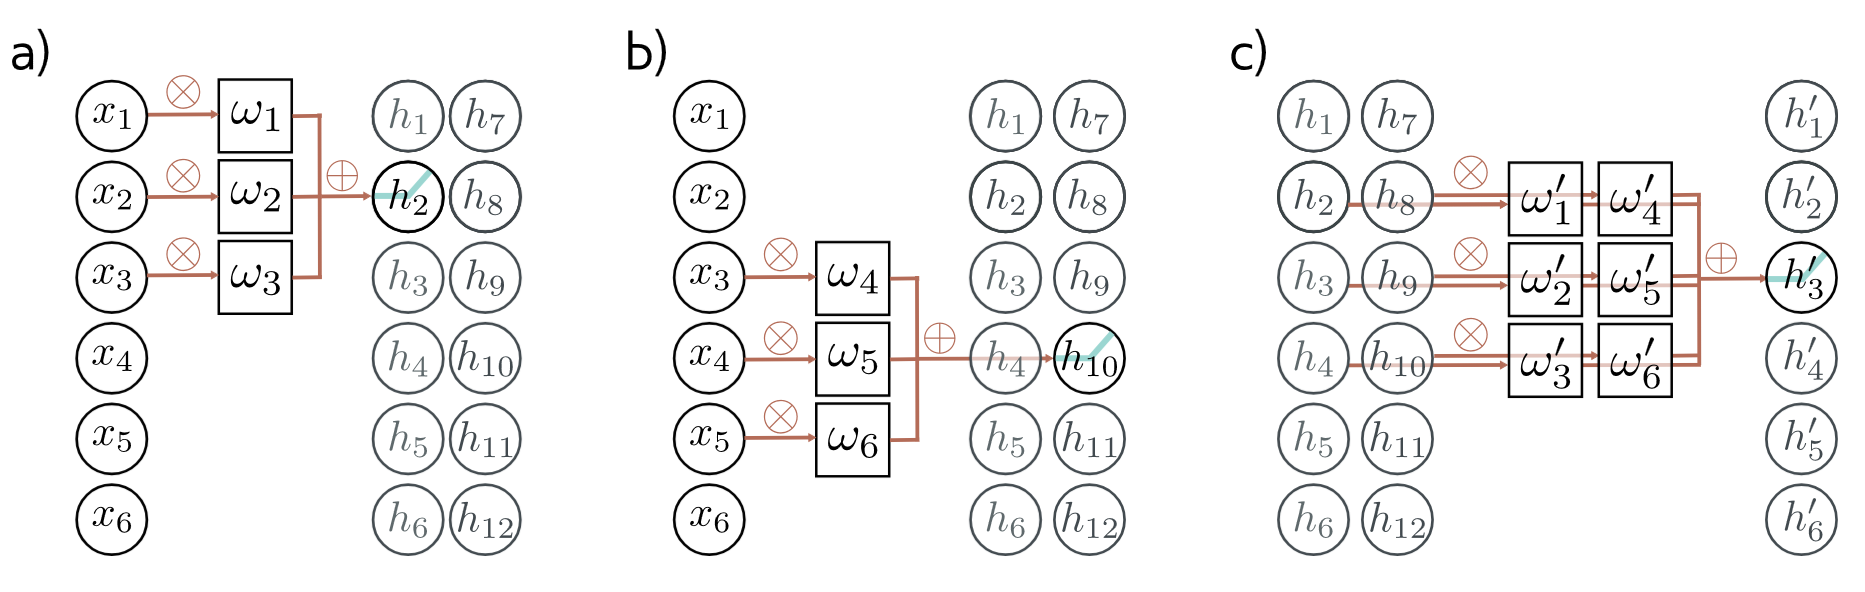
\includegraphics[width=0.8\textwidth]{img/8-kernel_applications.png}
    \caption{Channels. Typically multiple convolutions are applied to the input $\mathbf{x}$ and stored in channels. (a) A convolution is applied to create hidden units $h_1$ to $h_6$, which form the first channel. (b) A second convolution operation is applied to create hidden units $h_7$ to $h_{12}$, which form the second channel. The channels are stored in a 2D array $\mathbf{H}_1$ that contains all the hidden units in the first hidden layer. (c) If we add a second convolutional layer, then there is now one hidden unit per channel at each input position. The convolution kernel now defines a weighted sum over all of the input channels at the three closest positions to create each new output channel. If the input has $C_i$ channels and the kernel size is $K$, then there will be $C_i \times K$ weights and one bias needed to create each of the $C_o$ output channels. This makes a total of $C_i \times C_o \times K$ weights and $C_o$ biases.}
\end{figure}

\begin{figure}[H]
    \begin{minipage}{0.5\textwidth}
        \centering
        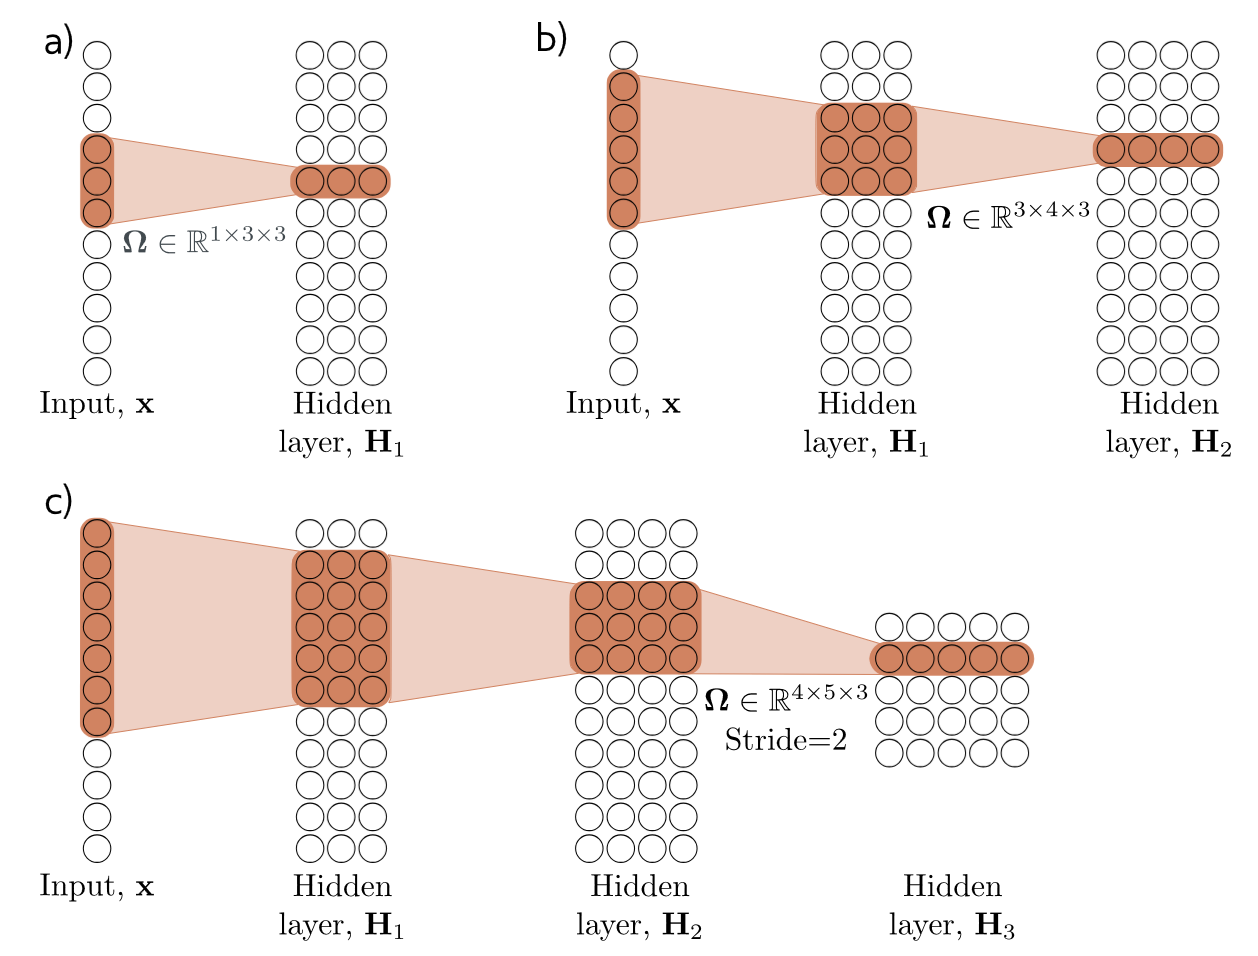
\includegraphics[width=0.8\textwidth]{img/8-width_depth.png}
    \end{minipage}
    \hfill
    \begin{minipage}{0.45\textwidth}
        \caption{Three-panel diagram illustrating Width and Depth. It shows how subsequent layers (Input $\rightarrow$ Hidden $H_1$ $\rightarrow$ Hidden $H_2$) integrate geometrically expanding overlapping regions (the orange cone expanding backwards to show the receptive field), highlighting how strides reduce the spatial dimension while kernels increase the depth dimension.}
    \end{minipage}
\end{figure}

\subsubsection{The Final Layer as a Processing Function}

Ultimately, a CNN acts as a sophisticated, multi-scale "processing function" of the initial input data. After the input has passed through numerous convolutional and pooling layers, the highly abstract, high-dimensional output tensor is typically flattened. The final layer of the architecture is almost always a standard feedforward, fully connected neural network. This dense layer analyzes the extracted topological features to execute the final predictive task, such as numerical regression or categorical classification.

\begin{figure}[H]
    \begin{minipage}{0.5\textwidth}
        \centering
        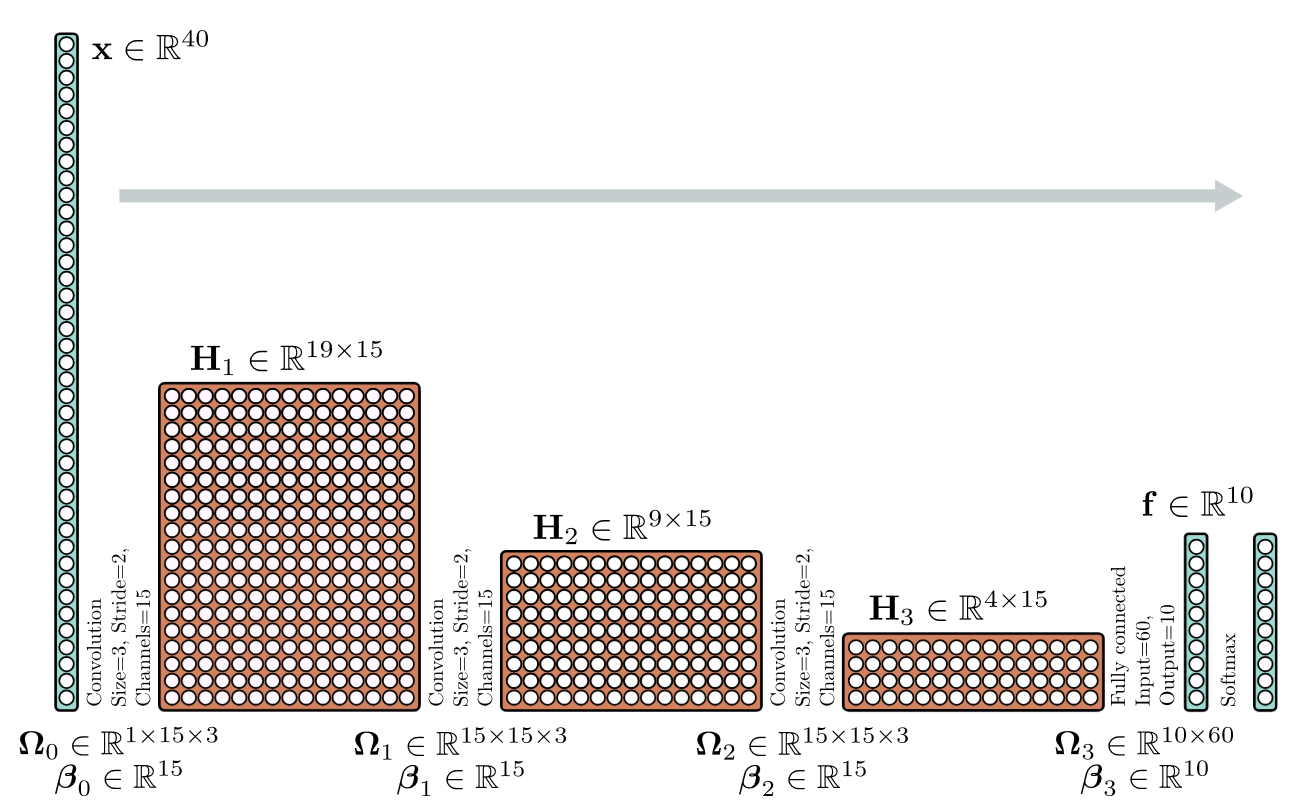
\includegraphics[width=0.9\textwidth]{img/8-cnn_architecture.png}
    \end{minipage}
    \hfill
    \begin{minipage}{0.45\textwidth}
        \caption{Schematic diagram of a full CNN architecture. The diagram illustrates a 1D input vector being passed through multiple convolutional blocks (e.g., $H_1, H_2, H_3$) with decreasing spatial dimensions and increasing channel depths, finally terminating in a flattened, fully connected feedforward layer leading to a Softmax output vector.}
    \end{minipage}
\end{figure}

\subsection{Graph Convolutional Neural Networks (GCNNs)}
\label{subsec:graph_convolutional_neural_networks}

Having established the mechanics of regular convolution, we can conceptualize an analogous process mapped directly onto complex networks, leading to the formulation of Graph Convolutional Neural Networks (GCNNs).

\subsubsection{Translating Convolution to Graphs}

In a GCNN framework, the fundamental components of a CNN are redefined for the graph domain:
\begin{itemize}
    \item \textbf{Input:} Instead of pixel intensities, the input consists of one or more continuous or discrete feature values ($x_i$) associated with each individual node $i$ in the network.
    \item \textbf{Filtering:} The application of a kernel is redefined as aggregating information over a specific \textit{subgraph}—most commonly, the immediate topological neighborhood of a target node.
    \item \textbf{Hierarchy:} The recursive application of these graph convolutions yields higher-level representations, strictly taking into account graph homomorphism relations to ensure structural integrity is maintained across layers.
\end{itemize}

\subsubsection{The Issue of Heterogeneity}

The primary mathematical hurdle in translating CNNs to GCNNs is topological irregularity. Vectors, matrices, and images constitute perfectly regular discrete lattices; every interior pixel in a 2D image has exactly 8 adjacent neighbors. This regularity allows for the application of a constant, fixed-size kernel matrix.

In stark contrast, real-world complex networks are inherently \textbf{non-homogeneous}. Node neighborhoods possess wildly varying sizes (degrees). A hub node might have thousands of neighbors, while a peripheral node might have only one. Consequently, it is mathematically impossible to apply a singular, fixed-size mathematical kernel across all nodes uniformly.

\subsubsection{Aggregating Node Information: Workarounds}

To overcome the issue of structural heterogeneity and properly aggregate node information, several methodological workarounds have been developed in modern GCNN architectures:

\begin{itemize}
    \item \textbf{Spatial Subsampling:} One approach is to artificially force homogeneity by sampling an \textbf{equal number} of neighbors for every node. If a node has too many neighbors, a random subset is sampled; if a node has too few, zero-padding or resampling is utilized. This spatial aggregation technique is the foundational principle behind algorithms like \textit{GraphSAGE}.
    \item \textbf{Spectral Transforms:} Alternatively, instead of operating directly in the irregular spatial domain, the convolution can be executed in the spectral domain. This involves applying a convolutional kernel to a mathematical \textbf{transform} of the network, utilizing tools such as the Laplacian spectral decomposition (a graph-theoretic analogue to the Fourier transform). By manipulating the eigenvalues and eigenvectors of the graph Laplacian, the network bypasses the need for fixed spatial kernels entirely.
\end{itemize}

\subsection{Spatial Aggregation Frameworks: GraphSAGE}
\label{subsec:spatial_aggregation_graphsage}

To address the heterogeneity of node degrees in spatial graph convolutions, frameworks like \textbf{GraphSAGE} (Sample and Aggregate) introduce a highly effective convolution-like approach. Instead of attempting to process the entire, irregularly shaped neighborhood of a node, GraphSAGE combines the feature vector of the target node ($x_i$) with a node neighborhood of a strictly \textit{fixed size}.

To achieve this fixed size, the neighborhood is \textit{randomly sampled} at each step of the training and testing phases. This localized convolution is applied iteratively up to the $k$-th neighbors, where $k$ represents the number of "hops" or search depth. A distinct set of learnable weight matrices $W$ is then used to concatenate and aggregate the outputs across these $k$ hierarchical levels into a single dense vector representation.

\begin{figure}[H]
    \centering
    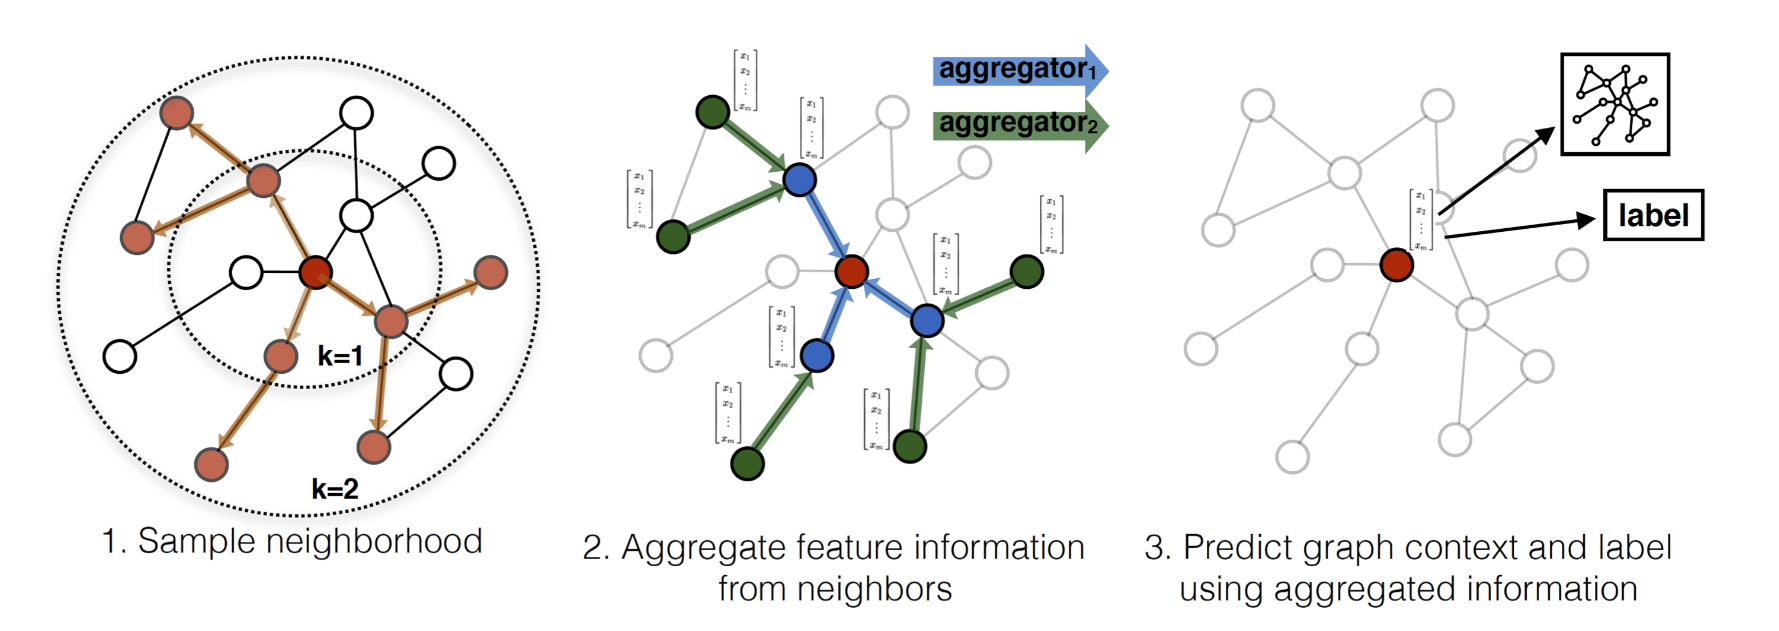
\includegraphics[width=0.8\textwidth]{img/8-graphsage.png}
    \caption{Schematic diagram illustrating the GraphSAGE methodology. The diagram is divided into three panels: (a) "Sample neighborhood" shows a target node with concentric circles representing $k=1$ and $k=2$ sampled neighbors; (b) "Aggregate feature information" illustrates vectors flowing from the neighbors to the target node through aggregator functions; (c) "Predict graph context and label" depicts the final aggregated embedding being used for downstream tasks.}
\end{figure}

\subsubsection{Unsupervised Training in GraphSAGE}

GraphSAGE can be trained using an unsupervised cost function, $J$, which optimizes the node embeddings $z_i$ by encouraging topological proximity. The objective is to maximize the similarity among representations of neighboring nodes while explicitly penalizing similarity among non-neighboring nodes.

The loss function for a target node $u$ is formally defined as:
$$J_{\mathcal{G}}(z_u) = -\log \left( \sigma(z_u^\top z_v) \right) - Q \cdot \mathbb{E}_{v_n \sim P_n(v)} \log \left( \sigma(-z_u^\top z_{v_n}) \right)$$

This equation consists of two competing terms:
\begin{itemize}
    \item \textbf{The Similarity Term:} The first term focuses on the similarity between the embedding of node $u$ and node $v$, where $v$ is a neighbor reached via a random walk of a fixed, identical length. This represents the positive sampling of connectivity paths.
    \item \textbf{The Dissimilarity Term:} The second term represents a negative sampling function. It evaluates the expected value over negative examples $v_n$ (drawn from a negative sampling distribution $P_n$), forcing the embeddings of non-neighbor nodes to diverge in the vector space, scaled by a factor $Q$.
\end{itemize}

\subsubsection{Inductive Capability and Structure Independence}

A profound advantage of the GraphSAGE architecture is that the training process is largely independent of the macroscopic network structure. Because the algorithm relies on the uniform random subsampling of local neighborhoods and learns aggregation \textit{functions} rather than fixed topological matrices, it exhibits strong inductive capabilities.

Consequently, training can be performed on a \textit{single network instance} (for example, a specific protein-protein interaction network). Once the aggregator weights and masks are learned, the trained model can be directly \textit{applied} to entirely different, unseen networks. For instance, a model trained on human protein interactions can be used to generate embeddings for the protein networks of different organisms, or even translated to distinct topologies like citation or social networks, precisely because the learned masks are network-structure independent.

\subsection{Spectral GCNNs and the Fourier-Like Transform}
\label{subsec:spectral_gcnns}

An alternative to the spatial sampling approach is to execute the convolution in the spectral domain. In this paradigm, the feature vector associated with the nodes (which can contain scalar values or multi-dimensional vectors for each node) is integrated using a CNN approach only \textit{after} applying a mathematical transform at the whole-network level. This ensures that the global information about the network structure is inherently embedded within the transform itself.

\subsubsection{Laplacian Spectrum as a Fourier Basis}

The mathematical solution relies on the normalized graph Laplacian matrix ($L$) and its spectral decomposition. By projecting the raw node features onto the orthogonal eigenvector basis of the Laplacian operator, we effectively translate the graph signal into the spectral domain. Convolution is then safely applied to this resulting transformed node feature vector using standard operations (e.g., scalar products).

This process is fundamentally analogous to a discrete Fourier Transform. In a standard 1D continuous lattice, the continuous Fourier transform is defined as:
$$\mathcal{F}(v_i) = \int e^{-iv_i x} f(x) dx$$

When discretized for a network manifold, the eigenvector basis of the Laplacian corresponds directly to discretized versions of stationary periodic functions (i.e., discrete sine and cosine waves oscillating at specific frequencies dictated by the eigenvalues). The discrete, graph-based Fourier transform can be conceptualized as:
$$\mathcal{F}(v_i) = \sum_j \sin(v_i \cdot x_j) \cdot x_j$$

In strict linear algebra terms, applying the Laplacian eigenvector matrix $U$ to the node feature vector $\vec{x}$ executes this Fourier transform on the manifold provided by the network structure:
$$\vec{\mathcal{F}} = U \cdot \vec{x} \quad \text{where} \quad L = U^\top \Lambda U$$

\subsubsection{Dimensionality and Empirical Applications}

The size of the Fourier-transformed space—which serves as the direct input to the convolutional layers—depends strictly on the type and number of Laplacian eigenvectors chosen for the projection. The maximum possible dimension equals the total number of nodes in the graph, though typically a truncated subset of the lowest-frequency eigenvectors is used to capture smooth macroscopic structures while filtering out high-frequency noise.

In this spectral setup, each entire network instance acts as a single input sample for training. Prominent empirical applications include:
\begin{itemize}
    \item \textbf{Neuroscience:} Analyzing brain connectome networks (anatomical or functional) where the node features are NMR/fMRI voxel intensities for a set of patients.
    \item \textbf{Bioinformatics:} Evaluating protein interaction networks where the node features represent protein or mRNA expression levels for individual patients.
\end{itemize}
These models are exceptionally powerful for case-control studies, complex sample classification, and parameter estimation via regression (e.g., predicting a patient's age based on their functional connectome).

\subsection{Biologically Informed Neural Networks (BINNs)}
\label{subsec:binns}

Standard fully connected neural networks treat their internal topology as a "black box" optimization problem. However, in many scientific disciplines, the underlying structure of the data is already well documented. \textbf{Biologically Informed Neural Networks (BINNs)} leverage this prior knowledge by building feedforward neural architectures whose exact wiring diagram is dictated entirely by an empirical biological network.

\subsubsection{Information-Driven Architecture}

A prime example is the analysis of proteomic data from case-control patient studies. Instead of a dense, fully connected hidden layer, the data is embedded into a sparse neural network whose architecture maps perfectly to the REACTOME metabolic reaction network (a directed graph of biological pathways). A link in the neural network only exists if an element is formally part of a specific biological reaction or pathway.

Typically, these BINNs utilize a multi-scale, hierarchical organization containing distinct layers, such as:
\begin{enumerate}
    \item \textbf{Proteins} (Raw input layer)
    \item \textbf{Basic Pathways} (First hidden layer)
    \item \textbf{Higher-order Meta-Pathways} (Second hidden layer)
    \item \textbf{Biological Functions \& Processes} (Final abstraction layer before classification)
\end{enumerate}

\begin{figure}[H]
    \centering
    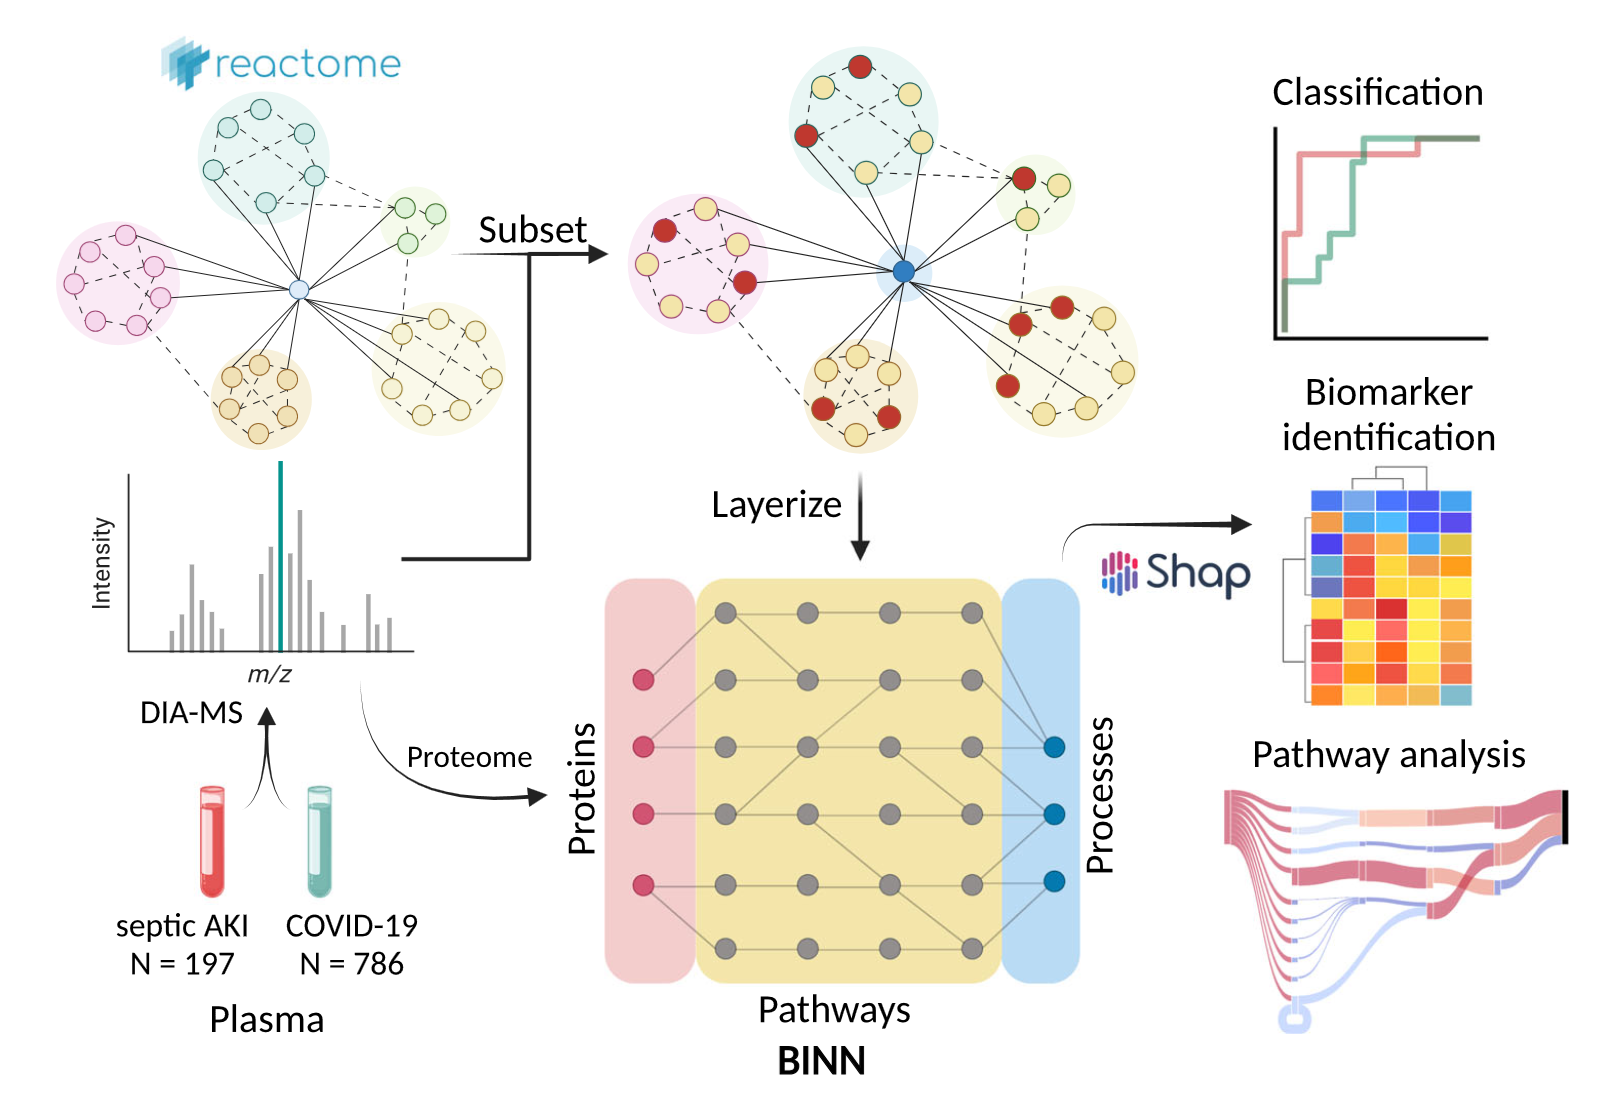
\includegraphics[width=0.8\textwidth]{img/8-binn_architecture.png}
    \caption{Schematic diagram illustrating the architecture of a Biologically Informed Neural Network (BINN). The diagram shows mass spectrometry plasma data from case/control groups feeding into a hierarchical neural network. The hidden layers are explicitly labeled as "Proteins", "Pathways", and "Processes", with the connections mimicking a biological reactome network, ultimately leading to classification, pathway analysis, and biomarker identification.}
\end{figure}

\subsubsection{Advantages and Explainability}

BINNs offer several profound architectural advantages:
\begin{itemize}
    \item \textbf{Reduced Parameter Space:} By forcing sparsity based on actual biological connections, the number of learnable parameters (weights) is drastically reduced, mitigating overfitting on small biomedical datasets.
    \item \textbf{Structural Hyperparameters:} The information-driven architecture turns the network structure itself into a hyperparameter, explicitly embedding centuries of biological research into the deep learning model.
    \item \textbf{High Explainability:} Because every hidden neuron represents a known biological entity (e.g., a specific metabolic pathway), researchers can interpret the exact role of different network elements in the final prediction. This is typically evaluated using the \textbf{SHAP (SHapley Additive exPlanations)} method, where one node is computationally removed at a time, and the subsequent drop in model performance is evaluated to quantify that specific node's biological relevance (often rescaled based on the logarithm of the number of downstream nodes reached).
\end{itemize}